% Este arquivo .tex será incluído no arquivo .tex principal. Não é preciso
% declarar nenhum cabeçalho
\section{Serviços da Unicamp}
\subsection{Atendimento médico e odontológico -- CECOM}

A CSS é responsável pelo planejamento e execução de programas de saúde voltados
à comunidade universitária da Unicamp -- alunos, funcionários e docentes.
É responsável também pelo atendimento à saúde oral desta comunidade, incluindo
também os filhos menores de servidores que estejam devidamente matriculados nas
creches e escolas dos campi.

Em português, isso quer dizer que é um ``plano de saúde'' da Unicamp. Demora um
pouco (embora o pronto-socorro do CECOM seja bem mais rápido que o do HC), tem
burocracia, mas funciona. Você pode marcar consultas médicas e fazer exames.
O CECOM é localizado próximo ao HC. Para ir, é melhor pegar o Circular pois
é beeeeeem longe. De circular interno, peça para descer no CECOM. É o ponto
final ou o penúltimo dos circulares.

Caso você tenha Unimed, o Centro Médico, que fica perto da Unicamp, atende pela
Unimed. É mais rápido que o atendimento da Unicamp (CECOM ou SUS).

%%% Imagem do hospital
\begin{figure}[h!]
    \centering
    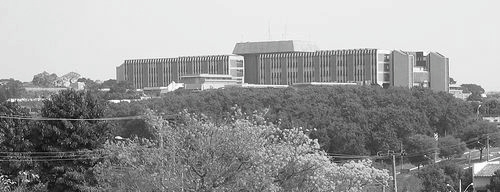
\includegraphics[scale=0.60, keepaspectratio=true]{img/imgs/13-servicos_unicamp/-077.jpg}
    \caption{Vista do Hospital de Clínicas da Unicamp}
\end{figure}


Para marcar consultas com Dentista, vá ao CECOM e pergunte onde que é. Isso é mais
fácil que você tentar entender lendo aqui. Basicamente é embaixo do CECOM, muito
fácil de chegar se alguém apontar com e dedo e dizer ``ali''. Funciona muito bem,
o atendimento é ótimo. A única burocracia é assistir uma palestra sobre doenças
da boca e escovação antes de poder marcar atendimento. Mas se você estiver com
dores eles te atendem na hora sem marcar consulta nem assistir palestra.

Para saber mais sobre o CECOM, vá ao site deles
(\url{www.unicamp.brcss/}).

\subsection{Hemocentro}

Essa é para quem é (ou para quem quer ser) doador de sangue. O centro de
hematologia e hemoterapia (hemocentro) é o órgão da Unicamp responsável pela
coleta e doação de sangue.
\begin{wrapfigure}{r}{0.2\textwidth}
    \vspace{-20pt}
    \begin{center}
    
\includegraphics[scale=0.14, keepaspectratio=true]{img/imgs/13-servicos_unicamp/doe_sangue2.jpg}
    \end{center}
    \vspace{-20pt}
\end{wrapfigure}
Qualquer pessoa pode aparecer no hemocentro para
fazer a doação de sangue. Basta estar com o RG e seguir um conjunto de normas
para a doação de sangue. Para saber mais sobre o processo, é só visitar a página
do hemocentro (\url{www.hemocentro.unicamp.br}).


O hemocentro também faz o projeto doador universitário, que consiste de unidades
móveis (ônibus) que param em alguns pontos do campus. Essas unidades fazem
a coleta do sangue. Alunos, professores e funcionários podem ir até essas
unidades móveis para fazer a doação. Para se informar melhor, é só visitar
a página do projeto
(\url{www.cecom.unicamp.brdoador_universitario/doador_universitario.html}).

O hemocentro fica localizado acima do HC (próxima ao CECOM). Portanto, se quiser
se deslocar até lá, como está escrito acima, é melhor usar o circular interno.

\subsection{Circular Interno e Ônibus Moradia}

O \textbf{Circular Interno} é um serviço de ônibus gratuito que dá voltas na Unicamp. Há duas linhas,
uma girando no sentido horário e outra no anti-horário. Só funciona até às 19h,
e a frequência maior é no horário de almoço. Bom para cobrir distâncias
como bandejão--IC, IC--FEEC, qualquer lugar--CECOM, qualquer lugar--FEAGRI,
FEAGRI--qualquer lugar. Quase todos os pontos têm os itinerários e os horários afixados.
Ele não costuma atrasar nem adiantar mais que 5 minutos, exceto no período de
férias.

O \textbf{Circular Noturno} é um ônibus que dá uma volta na Unicamp partindo do balão da
Avenida 1, passando pela BC, IQ, FEEC, IC e voltando para o balão da Avenida 1.
Os horários e o itinerário desse ônibus não estão nos pontos como os do Circular
Interno 1 e do 2. Ele funciona das 19h às 23h, a cada meia hora.

O \textbf{Ônibus Moradia} (ou ``Circular Externo'') dá uma volta na Unicamp partindo da BC, vai
para a Moradia e faz o caminho contrário. Ele também tem duas rotas alternativas
em horários específicos que cobrem as regiões da Avenida 1, Centro de Barão Geraldo
e Avenida 3. Os horários mais lotados do Ônibus Moradia são 8 da
manhã (sentido Moradia--Unicamp), horário de almoço (ambos os sentidos), horário
de jantar (ambos os sentidos) e o último horário (Unicamp--Moradia). Se puder
evitar esses horários, faça-o.

Todos os itinerários e horários detalhados dos serviços de ônibus podem ser
encontrados na página da Prefeitura da Unicamp: \url{prefeitura.unicamp.br}.

\subsection{SAE -- Serviço de Apoio ao Estudante}

O SAE (Serviço de Apoio ao Estudante), principal órgão de apoio ao estudante na
Unicamp, 
\begin{wrapfigure}{l}{0.22\textwidth}
    \vspace{-20pt}
    \begin{center}
    
\includegraphics[scale=0.65, keepaspectratio=true]{img/imgs/13-servicos_unicamp/-081.jpg}
    \end{center}
    \vspace{-20pt}
\end{wrapfigure}
atua em várias frentes de assistência estudantil. Esta se dá por meio
do gerenciamento de bolsas-auxílio, assistência social e orientações
educacional, jurídica e psicológica, além de apoio a projetos acadêmicos
e sociais e programa de intercâmbio de estudantes no exterior. O SAE também
é responsável pela gestão de estágios na Universidade.

\begin{itemize}
\item  Localização: Prédio do Ciclo Básico, 3º piso (responsável pelo gerenciamento de convênios, estágios, bolsa-pesquisa e bolsa-empresa); e em frente a DAC (serviço social, responsável pelo gerenciamento de bolsas-auxílio).
\begin{itemize}
\item  Horário: Segunda a sexta, das 08h30 às 20h, no período letivo.
\item  Contato: sae [@] unicamp [.] br
\item  Site: \url{www.sae.unicamp.br}
\end{itemize}
\end{itemize}

\subsection{Bolsas-Auxílio}
\subsubsection{Moradia}

Criado em 1989, o Conjunto Residencial Universitário da Unicamp, tem por
finalidade garantir estadia gratuita e de qualidade para os estudantes que
passam por dificuldades sócio-econômicas.

Para saber mais sobre o processo seletivo entre no site da Moradia da Unicamp
(\url{www.prg.unicamp.brmoradia/index.html}).

\subsubsection{Bolsa Alimentação e Transporte}

Objetivo: Colaborar com o estudante de graduação e pós-graduação em dificuldade
sócio-econômica, nos itens alimentação e transporte.

Critérios para a seleção: Análise do questionário sócio-econômico devidamente
preenchido e documentado, e entrevista com a assistente social.

\subsubsection{Bolsa Trabalho}

Objetivo: Colaborar com o estudante de graduação em dificuldade sócio-econômica,
cuja família não tenha condições de mantê-lo na Universidade. Em contrapartida
o bolsista trabalhará 15 horas semanais em unidades da Unicamp, ou em grupos de
pesquisas, ou em grupos sociais, em horário compatível com o horário escolar.
E com a orientação de um professor.

Critérios para a seleção: Análise do questionário sócio-econômico devidamente
preenchido e documentado, e entrevista com a assistente social.

Alunos da pós não podem se candidatar à bolsa trabalho.

\subsubsection{Bolsa Emergência}

Objetivo: Atender os estudantes de graduação regularmente matriculados que
estejam passando por dificuldades econômicas emergenciais. Em contrapartida
o bolsista trabalhará 40 horas em unidades da Unicamp, compatível com o horário
escolar.

Procedimento: o candidato deverá enviar uma carta à Coordenação do SAE
solicitando o benefício e informando sobre os motivos. Preencher e entregar
devidamente documentado o questionário sócio-econômico e marcar entrevista com
a assistente social.

Critérios para seleção: Análise da solicitação, do questionário sócio-econômico
devidamente preenchido, documentado e entrevista com a assistente social.

Alunos da pós não podem se candidatar à bolsa emergência.

\subsubsection{Bolsa PAPI}

Busca incentivar a participação de alunos de graduação e de pós-graduação nas
mais diversas atividades da Unicamp, tais como no auxílio a eventos. Neste
programa, há a solicitação de estudantes por parte de alguma Unidade ou órgão da
Unicamp, que poderá indicar o nome do aluno ou deixar a critério do SAE para
fazê-lo.

\subsection{Assistência Jurídica}

Objetivo: Orientar os alunos nacionais ou estrangeiros de graduação ou
pós-graduação, na resolução de suas questões pessoais de cunho jurídico que
envolvam os ramos do Direito, principalmente os seguintes:

\begin{itemize}
\item  \textbf{Direito Civil:} contratos em geral; contratos de locação de imóvel/escritura de compromisso de venda e compra; acidentes de trânsito; reparação de dano; ação revisional de aluguel; separação judicial; divórcio; pensão alimentícia, etc.
\item  \textbf{Direito Penal:} violência contra a pessoa; lesões corporais; furto; roubo etc{\dots}
\item  \textbf{Direito do Trabalho:} caracterização de relação de emprego para os não registrados e direitos trabalhistas em geral (Normas da CLT).
\end{itemize}

Procedimento: O aluno deve dirigir-se pessoalmente ao SAE para obter os
esclarecimentos desejados.

Delitos de consumo, encaminhar ao SEDECON ou ao PROCON.

Com relação aos contratos de locação alertamos para algumas dicas importantes:

\begin{itemize}
\item  Jamais pagar qualquer valor antecipadamente (ex: ``taxas de reserva de imóvel'', ``taxa de contrato'', aluguel antecipado etc), ou fornecer títulos em garantia: (cheque pré-datado, nota promissória).
\item  Obter o maior número de informações possíveis relativas ao imóvel, proprietário(s), imobiliária, procuradores;
\item  Condições e valores para pagamento (aluguel e outros encargos ex.: Condomínio, IPTU, seguros etc, para uma real visualização do valor total a ser despendido).
\item  Sempre solicitar uma Minuta do contrato locação.
\item  Não assinar contrato ou qualquer outro documento antes de apresentá-lo para análise por um dos advogados da O.J. SAE.
\end{itemize}

\subsection{Orientação psicológica}

Objetivo: Prestar atendimento psicológico ao aluno de graduação, pós-graduação
e especial.

O Serviço de Orientação Psicológica do SAE funciona em associação com o Serviço
de Atendimento Psicológico e Psiquiátrico ao Estudante (SAPPE) do Departamento
de Psicologia Médica e Psiquiatria da FCM, desde a sua implantação, em 1987.

Funcionamento e informações:

\begin{itemize}
\item  Existem horários para consultas imediatas (ideais para quem está prestes a expulsar um amigo da república etc);
\item  O tratamento de longo prazo é obtido mediante uma palestra explicativa, um horário de atendimento individual e espera em uma lista de candidatos -- horários disponíveis e motivos especiais podem facilitar seu ingresso, mas lembre-se: não é porque aparentemente não parece importante o motivo pelo qual você procura ajuda que isso não deva ser levado a sério. Em alguns casos, apenas quatro seções são suficientes para a pessoa sair do tratamento (lembrando que ele pode ser interrompido a qualquer momento);
\item  Há possibilidade de tratamento em grupo terapêutico, psicoterapia individual, de família e de casal com uma das psicólogas da equipe. O grupo terapêutico é formado levando-se em conta que não devem haver pessoas muito próximas em sua formação, como condição de que o paciente tenha liberdade para falar de seus problemas com menos receio.
\end{itemize}

\subsection{Cadastro de veículos}

Para você poder entrar e sair da Unicamp sem ter de parar receber e entregar
o papel de identificação do veículo você pode cadastrar seu carro junto
à Prefeitura do Campus. O cadastramento do veículo deverá ser feito diretamente
na Central de Informações (próximo ao Balão da avenida 1) de segunda
a sexta-feira das 09h às 17h.

Documentos necessários:

\begin{itemize}
\item  Identidade funcional (para funcionários/docentes), identidade estudantil para alunos, carta de apresentação da unidade para estagiários;
\item  Documento do veículo;
\item  Preenchimento de declaração.
\end{itemize}
Há possibilidade de se cadastrar até três veículos, com um custo de R\$ 5,00
para o segundo e de R\$ 10,00 para o terceiro veículo.

\subsection{Licenças de Software Gratuitas}

Bixo, agora que você é um computeiro de verdade, sua responsabilidade de não
usar software pirata é ainda maior. Afinal de contas, em poucos anos você pode
estar do lado dos desenvolvedores -- e não apenas consumidores -- de software.

A vantagem é que, por estar na Unicamp, você agora tem acesso a várias
licenças gratuitas de software proprietário especiais para estudantes.

O LMS (Laboratório Microsoft) ligado ao Instituto de Computação oferece download
gratuito de uma grande variedade de software da Microsoft, como o sistema
\textbf{Windows} e o ambiente de desenvolvimento integrado (leia-se: serve para
programar) \textbf{Visual Studio}. O Office não está disponível. Para mais informações
sobre como se cadastrar e baixar, acesse: \url{www.lms.ic.unicamp.br}.

A CTIC (Coordenadoria de Tecnologia da Informação e Comunicação) obtém licenças
de muitos pacotes de software e disponibiliza para a comunidade acadêmica, inclusive
alunos. As aplicações de computação científica \textbf{Wolfram Mathematica} e \textbf{MATLAB} estão disponíveis
gratuitamente. Para mais informações, acesse: \url{www.ctic.unicamp.br/softwares}.

A multinacional Autodesk oferece licenças de estudante gratuitas para muitos de
seus programas, incluindo o \textbf{AutoCAD} e a aplicação de modelagem
3D \textbf{Maya}. Para baixar, cadastre-se usando seu e-mail da DAC, do IC ou da
FEEC em \url{students.autodesk.com}.